\chapter{\IfLanguageName{dutch}{Stand van zaken}{State of the art}}%
\label{ch:stand-van-zaken}

% Tip: Begin elk hoofdstuk met een paragraaf inleiding die beschrijft hoe
% dit hoofdstuk past binnen het geheel van de bachelorproef. Geef in het
% bijzonder aan wat de link is met het vorige en volgende hoofdstuk.

% Pas na deze inleidende paragraaf komt de eerste sectiehoofding.

% Dit hoofdstuk bevat je literatuurstudie. De inhoud gaat verder op de inleiding, maar zal het onderwerp van de bachelorproef *diepgaand* uitspitten. 
% De bedoeling is dat de lezer na lezing van dit hoofdstuk helemaal op de hoogte is van de huidige stand van zaken (state-of-the-art) in het onderzoeksdomein.
% Iemand die niet vertrouwd is met het onderwerp, weet nu voldoende om de rest van het verhaal te kunnen volgen, 
% zonder dat die er nog andere informatie moet over opzoeken \autocite{Pollefliet2011}.

% Je verwijst bij elke bewering die je doet, vakterm die je introduceert, enz.\ naar je bronnen. In \LaTeX{} kan dat met het commando \texttt{$\backslash${textcite\{\}}} of \texttt{$\backslash${autocite\{\}}}. Als argument van het commando geef je de ``sleutel'' van een ``record'' in een bibliografische databank in het Bib\LaTeX{}-formaat (een tekstbestand). Als je expliciet naar de auteur verwijst in de zin (narratieve referentie), gebruik je \texttt{$\backslash${}textcite\{\}}. Soms is de auteursnaam niet expliciet een onderdeel van de zin, dan gebruik je \texttt{$\backslash${}autocite\{\}} (referentie tussen haakjes). Dit gebruik je bv.~bij een citaat, of om in het bijschrift van een overgenomen afbeelding, broncode, tabel, enz. te verwijzen naar de bron. In de volgende paragraaf een voorbeeld van elk.

% \textcite{Knuth1998} schreef een van de standaardwerken over sorteer- en zoekalgoritmen. Experten zijn het erover eens dat cloud computing een interessante opportuniteit vormen, zowel voor gebruikers als voor dienstverleners op vlak van informatietechnologie~\autocite{Creeger2009}.

% Let er ook op: het \texttt{cite}-commando voor de punt, dus binnen de zin. Je verwijst meteen naar een bron in de eerste zin die erop gebaseerd is, dus niet pas op het einde van een paragraaf.

% \begin{figure}
%   \centering
%   \includegraphics[width=0.8\textwidth]{grail.jpg}
%   \caption[Voorbeeld figuur.]{\label{fig:grail}Voorbeeld van invoegen van een figuur. Zorg altijd voor een uitgebreid bijschrift dat de figuur volledig beschrijft zonder in de tekst te moeten gaan zoeken. Vergeet ook je bronvermelding niet!}
% \end{figure}

% \begin{listing}
%   \begin{minted}{python}
%     import pandas as pd
%     import seaborn as sns

%     penguins = sns.load_dataset('penguins')
%     sns.relplot(data=penguins, x="flipper_length_mm", y="bill_length_mm", hue="species")
%   \end{minted}
%   \caption[Voorbeeld codefragment]{Voorbeeld van het invoegen van een codefragment.}
% \end{listing}

% \lipsum[7-20]

% \begin{table}
%   \centering
%   \begin{tabular}{lcr}
%     \toprule
%     \textbf{Kolom 1} & \textbf{Kolom 2} & \textbf{Kolom 3} \\
%     $\alpha$         & $\beta$          & $\gamma$         \\
%     \midrule
%     A                & 10.230           & a                \\
%     B                & 45.678           & b                \\
%     C                & 99.987           & c                \\
%     \bottomrule
%   \end{tabular}
%   \caption[Voorbeeld tabel]{\label{tab:example}Voorbeeld van een tabel.}
% \end{table}
 
\section{Wat is een PLC}
Een PLC (Programmable Logic Controller) is een industriële computer die wordt gebruikt voor het automatiseren van machines en processen \autocite{Bolton2015}. 
Het is ontworpen om robuust te zijn en betrouwbaar te functioneren in industriële omgevingen zoals fabrieken, 
waar het vaak wordt gebruikt om mechanische apparatuur, zoals transport systemen of liften van een automatisch magazijn te besturen.

TODO: detailed information about current PLC system that is subject

\section{Wat is een WCS}
Warehouse control systemen (WCS) zijn softwaretoepassingen die bedrijven in staat stellen om magazijnactiviteiten te beheren en te controleren, 
waaronder voorraadbeheer, orderverwerking en transportbeheer. 
Warehouse control systemen vormen een essentieel onderdeel van moderne magazijnactiviteiten \autocite{Rana2023}. \newline

TODO: detailed information about current WCS system that is subject

\section{Communicatie tussen PLC en WMS}

\section{Soorten communicatie}


\section{Synchroon vs. asynchroon}
Services communiceren zowel \emph{synchroon} als \emph{asynchroon} en spelen deze benaderingen een cruciale rol, 
elk met hun eigen voor- en nadelen. \emph{Synchrone microservices} werken volgens een direct 
afhankelijkheidsmodel, omdat services met elkaar communiceren in een vraag-antwoordpatroon. 
Deze synchrone communicatie kan leiden tot ingewikkelde onderlinge afhankelijkheden, vertragingen en complexiteiten bij het debuggen 
van de logica. Bovendien wordt het schalen van synchrone microservices uitdagend, 
aangezien de schaalbaarheid van één service sterk afhankelijk is van andere services die het gebruikt \autocite{Bellemare2020}. 
\newline

Daartegenover bieden \emph{asynchrone microservices} een reeks voordelen. Ze bieden grotere schaalbaarheid, technologische 
flexibiliteit en aanpassingsvermogen aan veranderende zakelijke vereisten. 
In plaats van de synchrone manier van communicatie zijn \emph{asynchrone microservices} 
gemakkelijker te herstructureren en te onderhouden. 
Ze vergemakkelijken \emph{continuous delivery} door hun onafhankelijkheid omdat de communicatie 
met een \emph{messaging systeem} opgevangen wordt. Hun verminderde afhankelijkheden en 
geïsoleerde karakter maken het testen relatief eenvoudiger en robuuster.
Het enige grote nadeel in asynchrone communicatie is \emph{error handling}, 
omdat dit niet opgevangen kan worden door de verzendende partij.
\newline

\begin{figure}[H]
  \centering
  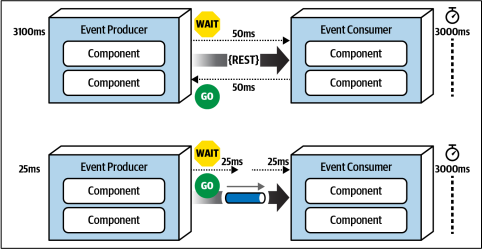
\includegraphics[width=.5\textwidth]{../voorstel/img/synchronous_vs_async_calls.png}
  \caption{\label{fig:img}Synchronous versus asynchronous communication \autocite[figure 14 -- 13]{MarkRichards2021}.}
\end{figure}

In praktische termen is het vinden van de juiste balans tussen synchrone en \emph{asynchrone microservices} cruciaal, 
afhankelijk van de specifieke behoeften van een organisatie en de aard van haar bedrijfsprocessen. 
Een hybride aanpak waarin beide architecturen naast elkaar bestaan en elkaar aanvullen blijkt vaak de meest effectieve strategie te zijn. 
Deze aanpak stelt organisaties in staat om de sterke punten van zowel synchrone als asynchrone modellen te benutten, 
waardoor flexibiliteit, schaalbaarheid en onderhoudsgemak worden gegarandeerd in complexe \newline IT-landschappen.
In deze paper ligt de focus op \emph{asynchrone communicatie} voor het gebruik van \emph{messaging systemen}.
\newline

\section{Overzicht Messaging Systeem}
Messaging systemen hebben dus een asynchrone werking en vallen onder \newline \emph{Inter-Process Communication (IPC)}. 
Deze systemen zijn \emph{socket-based} en maken gebruik van \emph{message queuing}, waarbij het de \emph{publish-subscribe} of de \emph{point-to-point} methodiek gebruikt \autocite{Dinari2020}. 
\newline
Een socketverbinding maakt gebruik van een endpoint gespecificeerd met een IP-adres en een \newline poortnummer, 
waarmee twee autonome processen verbonden zijn, hetzij op dezelfde, hetzij op verschillende machines.
\newline
\emph{Message Queuing} gebruikt deze manier van verbinden en maakt het voor applicaties mogelijk om asynchroon 
te communiceren zonder te moeten wachten op een antwoord van de ontvanger. 
Er zijn twee methodieken in deze systemen. 
\newline

De eerste methodiek is \emph{publish-subscribe}, waarbij de zender, genaamd \emph{publisher} niet verantwoordelijk is voor het beheer 
en het rechtstreeks verzenden van de berichten naar specifieke ontvangers, die \emph{subscribers} of abonnees worden genoemd. 
In plaats daarvan worden berichten door het messaging systeem of broker geclassificeerd en ter 
beschikking gesteld van de subscribers die ingetekend hebben op berichten uit een specifieke klasse.
Vervolgens ontvangen \emph{subscribers} berichten uit de klassen die voor hen interessant zijn, zonder dat ze kennis hebben van de \emph{publishers}.
Met het \emph{publish-subscribe-model} specificeert de afzender nooit expliciet de ontvanger,
hij weet zelfs niet of er wel of geen ontvanger bestaat.
\newline

\begin{figure}[h]
  \centering
  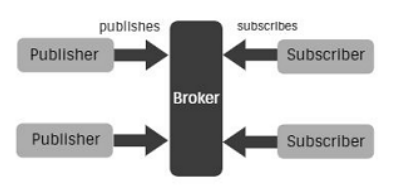
\includegraphics[width=.4\textwidth]{../voorstel/img/fig1-publish-subscribe.png}
  \caption{\label{fig:img}Publisher-Subscriber system\autocite{Sharvari2019}.}
\end{figure}

In dit model ontvangen \emph{subscribers} slechts een subset van de totale gepubliceerde berichten. 
Het proces van het selecteren en verwerken van de berichten wordt filtering genoemd. 
Er zijn twee vormen van filtering: op basis van onderwerp (topic) en op basis van inhoud (content).
\newline

In een op \emph{topic} gebaseerd systeem worden berichten geplaatst in \emph{topics} wat logische kanalen zijn.
\emph{Subscribers} ontvangen berichten van de \emph{topics} waarop ze zich hebben geabonneerd.
Alle \emph{subscribers} ontvangen dezelfde berichten uit dezelfde \emph{topics}. 
Deze methode zorgt voor een \emph{one-to-many} vorm van communicatie.
\newline

De tweede methodiek genaamd point-to-point gebruikt \emph{queuing} waarbij de \emph{producer} berichten plaatst in een specifieke queue, 
waarna een \emph{consumer} de berichten uitleest in een sequentiele volgorde. 
Met andere woorden, een bericht wordt slechts aan één \emph{consumer} bezorgt.


Een aantal onderzoeksvragen uit de probleemstelling dat deels kan worden beantwoord:

\begin{enumerate}

\item \textbf{Waarom is een weloverwogen keuze van essentieel belang?}
  \begin{itemize}
      \item Een weloverwogen keuze is essentieel omdat het huidige communicatie systeem inefficiëntie kan veroorzaaken en niet op modernere systemen 
      kan worden geïnstalleerd worden. Door zorgvuldig te kiezen kan dit probleem opgelost worden en een 
      efficiënter IT-landschap creëren.
  \end{itemize}

\item \textbf{Wat is de inspanning om een gekozen technologie te implementeren?}
  \begin{itemize}
      \item De inspanning om een gekozen technologie te implementeren kan variëren afhankelijk van de specifieke systeemvereisten, 
      de non-functional requirements en de beschikbare middelen binnen de organisatie. Dit kan onder meer het configureren, 
      aanpassen en integreren van de gekozen technologie omvatten, evenals het trainen van personeel en het uitvoeren van migraties van 
      bestaande systemen.
  \end{itemize}
\end{enumerate}



\section{Wat is een EoL systeem}

\section{Wat zijn de gevaren van EoL systemen}

\section{Welke manieren zijn er om EoL weg te werken}


